\numberedsection{RF5.2 Visualizar relación}

\subsection*{Descripción}
Permite a los usuarios visualizar una lista de categorías creadas en el sistema, incluyendo su nombre y el número de productos asociados a cada una.\par
\vspace{0.15cm}

\textbf{Pre-condición}\par
El usuario ha iniciado sesión en el sistema y se encuentra en el apartado de Categorías.\par
\vspace{0.15cm}

\textbf{Post-condición}
\begin{itemize}
    \item Caso de éxito: El sistema muestra la lista de categorías junto con el nombre y número de productos asociados.
    \item Caso mínimo: El sistema notifica al usuario el resultado de la acción de visualización de categorías: exitosa o fallida.
\end{itemize}

\textbf{Prioridad: }
Media
\vspace{0.15cm}

\textbf{Autor: }
Janine Bernadeth Olegario Laguit\par
\vspace{0.15cm}

\textbf{Control de cambios: } Versión 1: Definición del caso de uso

\numberedsubsection{Escenario principal}
\begin{enumerate}
    \item El usuario accede a la sección de gestión de categorías.
    \item El sistema muestra la lista de categorías existentes, incluyendo su nombre y el número de productos asociados.
\end{enumerate}

\numberedsubsection{Escenarios alternativos}
\begin{description}
    \item[2.a.] El sistema detecta que no existen categorías.
    \begin{enumerate}
        \item[2.a.1] El sistema muestra una lista vacía, con la opción de crear categorías nuevas.
    \end{enumerate}

\end{description}

\numberedsubsection{Casos de Prueba}
\underline{Escenario: Principal}\par
\vspace{0.15cm}

\textbf{Dado} que he iniciado sesión con mi cuenta de usuario correspondiente,\par
\textbf{Y} estoy en el apartado de Categorías,\par
\textbf{Entonces} el sistema muestra la lista de categorías existentes,\par
\textbf{Y} cada categoría se visualiza junto a su nombre y el número de productos asociados.\par


\vspace{0.20cm}

\underline{Escenario: Alternativo 2.a}\par
\vspace{0.15cm}

\textbf{Dado} que he iniciado sesión con mi cuenta de usuario correspondiente,\par
\textbf{Y} estoy en el apartado de Categorías,\par
\textbf{Y} no existen categorías registradas en el sistema,\par
\textbf{Entonces} el sistema muestra una lista vacía, con la opción de crear categorías nuevas.\par

\vspace{0.20cm}

\numberedsubsection{Bocetos}
\begin{figure}[H]
    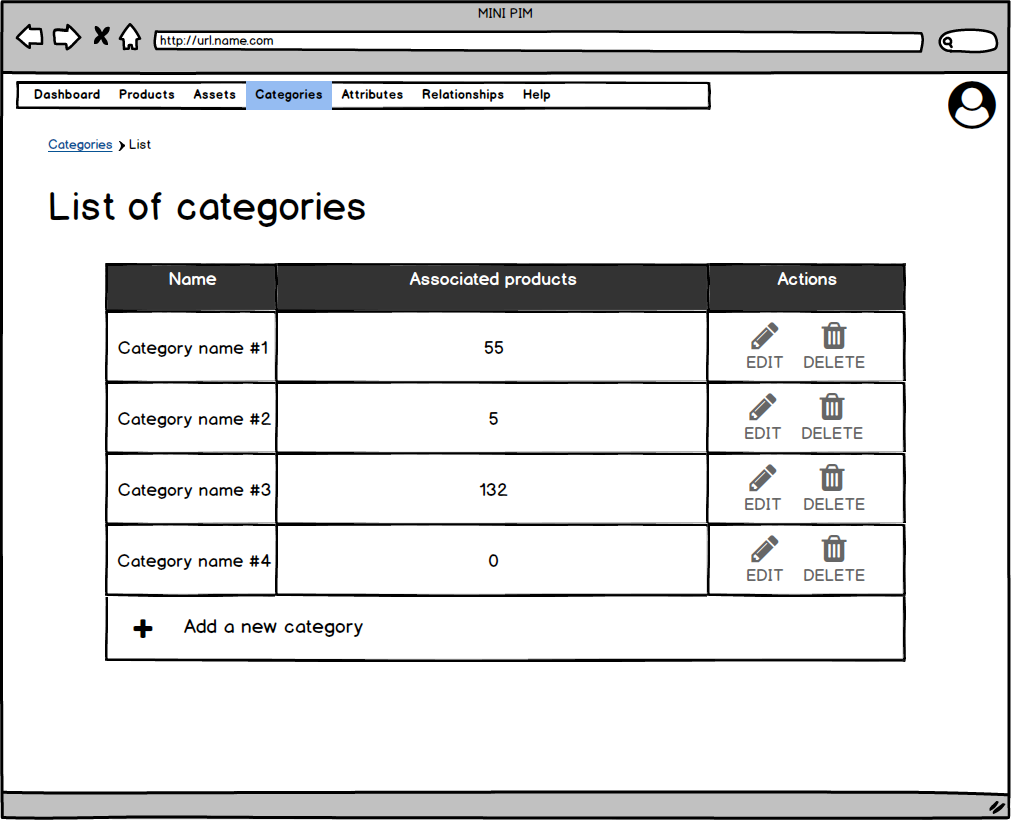
\includegraphics[width=1\linewidth]{mockups/RF4.2_1.png}
    \caption{Visualización de categorías}
   \end{figure}
\vspace{1.0cm}

\begin{figure}[H]
    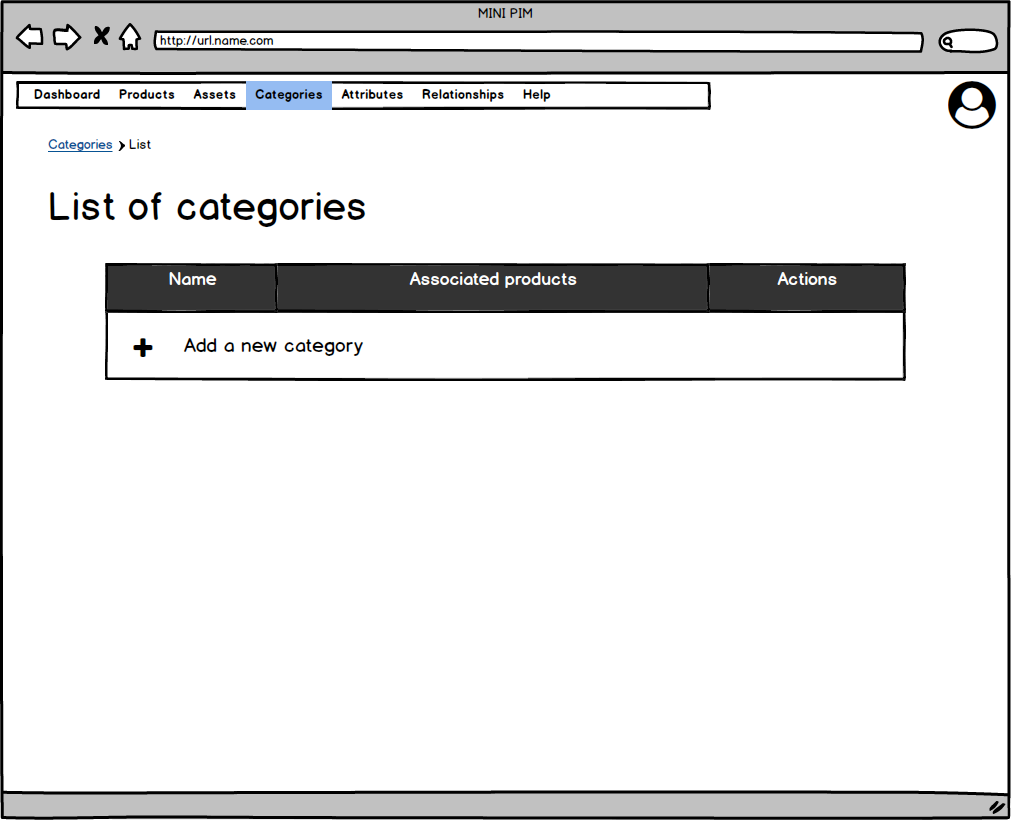
\includegraphics[width=1\linewidth]{mockups/RF4.2_2.png}
    \caption{Visualización de lista vacía}
   \end{figure}
\vspace{1.0cm}

\newpage % Nuevo caso de uso en nueva página